\section{Background and Motivation}
\label{background}

Artificial Intelligence (AI) is one of the fastest growing technology domains, involving academic research, businesses, and users. The enormous investment in AI led to groundbreaking applications in a diverse set of areas.  AI is used for accelerating the discovery of
drugs (e.g., \cite{stark2022equibind}, \cite{ross2022large}), driving efficiencies at work (e.g.,~\cite{puri2021codenet}), discovering new materials towards renewable storage (e.g.,~\cite{zitnick2020}), and more. 
At the same time, we are also in the midst of a heated debate about the potential of AI to harm (e.g., 
\cite{aidanger}). Risks frequently associated with AI include, fake news, biases, job losses, and, the enormous environmental cost. 

The amount of compute used to train deep learning models have increased $300,000\times$ in six years~\cite{schwartz2019green}. 
Data has increased significantly, reaching exabyte scale~\cite{Wu2022}. The data size increase has led to a super-linear growth trend in model size~\cite{Wu2022}. For example, $GPT3$ based language translation tasks have increased in size $1000\times$ (\cite{brown2020language}). In contrast, systems' memory
capacity only grew moderately,
%(e.g., NVIDIA A100 grew twice in size in a period of ~2 years), 
%The memory capacity of GPU-based accelerators, 
%e.g. $32GB$ NVIDIA V100 (2018) to $80GB$ NVIDIA A100 (2021) has increased by $< 2\times$ every $2$ years. The %resource requirements for strong AI scaling clearly outpaces that of system hardware, 
which has motivated a variety of scale-out infrastructure solutions (e.g.,~\cite{patterson2021carbon,Wu2022}), involving thousands of AI accelerators and other specialized systems. There is no doubt that these 
trends come with a dire environmental cost (stemming both from 
embodied and operational costs). Indeed, multiple researchers and practitioners have raised the alarm on the environmental cost of AI, and offered a calls-to-action (\cite{Strubell-policy-19,lacoste2019quantifying,Henderson2020Towards,schwartz2019green}). 
%For example, it is shown in  (\cite{Strubell2019}) that training a single large transformer model on a GPU device, can take up to the equivalent carbon of $5$ cars through their entire life time.

Meanwhile, a recent development in the field of AI, is foundation models (FMs) coming to the front stage (e.g., ~\cite{stanford-fm}). FMs are trained on very broad data-sets using self supervision at scale. One of the interesting characteristics of foundation models is that 
through transfer learning~\cite{thrun1998lifelong} they can be adapted (e.g., fine-tuned, or distilled) to a wide range of downstream tasks.  In fact, the majority of state-of- the-art NLP models are now adapted from one of a few foundation models, such as BERT~\cite{devlin2018bert}, RoBERTa ~\cite{liu2019roberta}, BART~\cite{lewis2019bart}, T5~\cite{raffel2020exploring}, BLOOM~\cite{workshop2023bloom}, LLaMA ~\cite{touvron2023llama}. 
Foundation models are not new, but the scale, scope, and emergent capabilities of foundation models in the last few years have exceeded everyone's imagination. For example, GPT-3 has $175$ billion parameters (in comparison with the `modest' $1.5$ billion parameters of GPT-2), and it can be adapted via natural language prompts to perform a range of tasks despite not being trained explicitly to do many of those tasks~\cite{brown2020language}. Proponents of foundation models claim that the enormous amount of upfront carbon cost to train a broad model is balanced in the `big picture' by the low cost of re-using it via fine-tuning or distillation for a particular task (e.g., \cite{stanford-fm}). 
Alas, with no unified metric that analyses the entire provenance chain of models, data-sets, and their associated cost, it is very hard to substantiate or refute this claim. 

In this position paper, we apply broad knowledge of sustainability principles, protocols and standards,
including the GHG Protocol (\cite{ghg-potoc}), and the accompanying guidance document for cloud services (\cite{ghg-guid}, chapter~$4$), and product Life Cycle Assessment principles (LCA)~\cite{lca},
to the domain of AI, in order to develop metric that can be meaningfully used to drive sustainability mindset and examine trade-offs across the life cycle of AI models, and across the `supply-chain' of models and data-sets.  
%and are measurable easy to calculate, reproducible, and useful. 
%
%Defenders of Foundation Models often claim that while the up-front environmental cost of training a Foundation Model is enormous, because they promote  low cost re-use at scale they contribute to reducing the overall global cost of AI. In order to analytically tackle this question, our metrics definition factors-in the entire 'supply chain' of models in defining the amortized cost of the actual unit of work performed, namely, the inference jobs submitted by end-user. 
%We believe that this approach can enable a more meaningful debate and selection of strategies ultimately leading to environmental harm reduction. 
%Our goal in this paper is to define metrics that can be used to evaluate AI efficiency {\em end-to-end} focusing on the end-user inference jobs as the main entity of interest and factoring in the entire 'supply chain' of models. We associating operational and embodied sustainability cost with end user driven inference jobs.
%
As in~\cite{gandhi2022metrics}, and also as in the Software Carbon Intensity (CSI) specification offered by the Green Software Foundation~\cite{GSF}, we focus on a unit of work submitted on behalf of an end-user, i.e., inference jobs in the case of AI, as the primary object of interest. The metric is meant to capture the actual amortized sustainability cost
of a job, taking into account operational overheads and associated embodied cost. 

We leverage and expand the metrics defined in~\cite{gandhi2022metrics}, concerning the sustainability cost of jobs. Specifically, 
We define and motivate a new term {\em Embodied Product Cost} for 
the sustainability cost of software, 
such as the development and testing of platforms delivered as 
an always running service (such as AWS's Lambda~\cite{lambda}), and, in the domain of AI, the preparing of data-sets, and training of models. We then expand the definition of job sustainability cost metrics ($JSC$ and $ASC$), to also 
factor in the associated embodied product cost. The expanded definition can contribute towards accuracy and completeness of job sustainability metrics.
We then show how to 
apply this expanded definition to the area of AI.  
%%
%%
%%Unfortunately, in our analysis, we reached a conclusion that one component is missing from the metric definition; which is, the cost of any software asset that is supporting the execution of the job being evaluated. 
%%Examples of such software assets include an always running platform service such as, the Lambda service~\cite{} to 
%%support the execution of Serverless jobs in AWS~\cite{}, 
%%or an AI model that is used to serve inference jobs.  In both cases, there is not only a significant operational overhead
%%to maintain the assets, 
%(such as the management components of a service that are always running, troubleshooting, and continuous development of an on-line platform service, or, continuous re-train of a model to maintain accuracy), 
%%there is also what we term 'embodied cost of software'; a concept which we introduce here for the first time to our knowledge, and which we adopted from its use for systems, to capture the energy and carbon cost to 'manufacture' the software asset, including development, testing, or training.
To summarize, 
the contribution of our paper is as follows: 
\begin{enumerate}
    \item We define a new metric {\em Embodied Product Cost}, that aims at expressing the `embodied' carbon of software assets,  i.e., the carbon cost of `manufacturing' a software asset, such as the development and testing of an on-line platform, or the pre-deployment training of an AI model. 
    \item We expand the definitions of Job Sustainability Cost ($JSC$), and 
    Amortized Sustainability cost ($ASC$), defined in~\cite{gandhi2022metrics} to factor-in the operational cost of the software asset used as the
    context of the execution of the job, as well as, the `embodied' costs of these software assets. The expanded 
    definitions can be used generally for any data center job, not just AI, and contribute towards accuracy and completeness.  
    \item We specialize and apply these new metrics to the case of AI. We show how our approach can promote a sustainability mind-set, and in particular can be used to analytically prove or refute the claim that foundations model re-use for downstream tasks is advantageous to the environment, relative to the construction of smaller more specific models, from scratch.
    \item We analyse the new opportunities for sustainability based research across the life-cycle and provenance chain of models.
    %Such as life-cycle strategies (e.g., use of Neural Architecture Search, or frequency of re-training, or re-use benefits), and 
    %trade-offs, based on requirements and expected use. 
\end{enumerate}

\subsection{Related Work}
Sustainable computing has gained significant attention since a decade ago, owing to the escalating demand for computing power in Cloud computing and hyper-scale data centers, which has resulted in a significant surge in energy consumption at the data center and energy proportional computing~\cite{dc_computer}. To address this concern, there have been continuous efforts aimed at reducing power/energy consumption across different levels, ranging from chip/HW components~\cite{jouppi2023tpu,jiang2020power,capra2020updated} to data center scale~\cite{7229319,7738551,7279063,9752582}, including cooling techniques (Power Usage Effectiveness, PUE) and/or total cost ownership (TCO)~\cite{ZHANG2021102253,mukherjee2020detailed,CHAUHAN2019450,ROSTIROLLA2022111787}. %PUE is ${total~facility~power}/{IT~equipment~energy}$, and TCO is ${I + M – R}$, where $I$ indicates the initial cost, and $M$ indicates the maintenance cost, and $R$ is the remaining value of the data center. These two metrics were a widely used metric to quantify the efficiency of data center. While it was initially projected that energy consumption would continue to increase at an alarming rate~\cite{epa},\cite{epa1}, many researchers agreed that this growth has been mitigated to some extent, as computer scientists, cloud service providers, data center managers, and software engineers have made remarkable efforts in enhancing energy efficiency of running their hardware and software. Nevertheless, the advent of AI (e.g., large language model and generative models) presents a fresh set of challenges.

%%\textbf{Tamar} 
Multiple recent works take a holistic view of the problem 
area of sustainability in computing. Gupta {\em et. al.}(~\cite{gupta2020chasing}) posits that
attention must be given to the embodied emission of systems, which is becoming the dominant 
factor in the carbon cost of computing environments. \cite{chien2020beyond} argues that 
we need to replace static metric such as PUE and grid emission factors (CI) with dynamic, time series based, metric to enable de-carbonization of data centers by co-optimization. We agree with these assertions and believe they are complementary to the approach presented here. The most relevant to this paper is the work by Gandhi {\em et. al.}~\cite{gandhi2022metrics} that argues that we should focus on the unit of work performed (namely, {\em a job}), and, include in its amortized sustainability cost also a `slice' of the embodied emission cost of the systems used for the execution and other operational overheads such as for cooling. This approach agrees with the software Carbon Intensity (SCI) specification~\cite{SCI}, put forward by the Green Software Foundations~\cite{GSF}. We agree that we should aim at amortizing all these aspects into the carbon sustainability cost of jobs. Toward that goal, we posit that we are neglecting to consider additional aspects associated with the {\em software product(s)} used as an execution context for the job. Examples of software products are a software platform, deployed as an always-running service, required for the execution of jobs (such as a serverless job running on the AWS Lambda platform service~\cite{lambda}), and, in the 
domain of AI, a model, that is used to serve inference requests initiated by end users. In both these cases there is a significant overhead associated with (1) the on-going maintenance of the product such as 
service operations, or, model continuous re-training, and, (2) the up-front construction of the product (including, development and testing, or, data preparation and training). We propose new metrics, that build on the previous ones, but include these two neglected factors. \\
%We then show how to apply these two metrics to the area of AI and analyze the benefits. We believe the sustainable computing community will ultimately benefit from a unified set of metrics. 
%
%%\textbf{* sustainable ai - MEta, FB, Green AI, Stadler? bruno - mo more pararaph (Tamar)}
In the area of AI, an astounding amount of progress has been accomplished on the systems side, to design energy efficient accelerators specifically for AI workloads, 
optimized for metrics multiplication, and incorporating low precision, and low voltage (e.g., ~\cite{7738674,888701}). Beyond 
the lens of system design, data scientists spend most of their attention 
fiercely competing over accuracy as a primary goal, and time-to-value as a secondary goals (e.g., ~\cite{liu2019roberta}). The papers ~\cite{Strubell-policy-19} and ~\cite{schwartz2019green}, were among the first to call attention to the issue of the environmental cost of AI, focusing in particularly, on the training phase of the life cycle. Michel {\it et. al.} \cite{Lenherr2021new}, offers a single metric that can be used to compare the energy efficiency of different models with respect to their complexity (e.g., based on number of classes), and their accuracy. The work~\cite{patterson2021carbon}, asserts the difficulty in assessing the $gC0_2e$ of AI models, which necessitate considering the energy mix in the location of the training, and the hardware architecture used. By considering these two aspect, they correct previous estimates, such as in~\cite{Strubell-policy-19} by as much as $88\times$.
%(specifically, of the $CO_2e$ cost for the neural architecture search for Evolved Transformer in ~\cite{ctr19} by a factor of $88\times$). 
They also join the call to define standards and norms for Sustainable AI. Lastly, Wu et. al~\cite{Wu2022}, is first to suggest we need
a {\em holistic} approach to Sustainable AI that considers {\em all stages
of the life cycle}, and also including the embodied emission of systems used. Some of the interesting findings in this paper are: (1) that the often completely overlooked data preparation phase, consumes in some cases an equal amount of energy as the training phase, and, (2) that the ratio between energy spent in different phases of the model life cycle  {\em varies across different use cases}. These two key observations contributed to motivating this position paper. First, we focus on two specific software assets: data-sets, and models. By defining the concept of `embodied emission of software' we capture the $gCO_2e$ cost of pre-preparation of data set, and 
pre-training of models. Further we factor-in these costs, as well as the, mostly overlooked, cost of maintaining a model with frequent re-training, in amortizing the $gCO_2e$ cost per inference transaction, which is the unit of work performed on behalf on an end user. We postulate that this  approach will allow us to analytically compare different 
strategies, e.g., the size of the model used, and whether it was distilled based on a previous model, or trained from scratch.  
%%\textbf{* ai optimization which is not energy related (bhatta) - not sure it is needed?}

\subsection{The life cycle of an AI model}
\label{life-cycle}
%% Introduce Foundation Models,  what are they and why we ought to think differently about 
%% the life cycle efficiency - how do we factor in re-use, model distelation, fine-tuning, and re-training? 
 %% Describe the model life cycle in details - all the stages ****plus a working example****
%A foundation model is a large artificial intelligence model trained on a vast quantity of data at scale (often by self-supervised learning or semi-supervised learning). It can be adapted to a wide range of downstream tasks ~\cite{stanford-fm}. 
%A majority of NLP models are now developed based on  a few foundation models, such as BERT, RoBERTa, BART, or, T5. It is projected ~\cite{stanford-fm} that foundation models will be developed across a wide range of modalities.
 To fully understand the real environmental impact, and to be able to develop the right approach to assess the impact, 
 we must closely examine the model life cycle, end-to-end, including: data collection, model exploration and experimentation, model training, model distillation, and fine tuning, deployment, and then re-training, and inference cost. 
%% \begin{figure*}[t]
%%\centerline{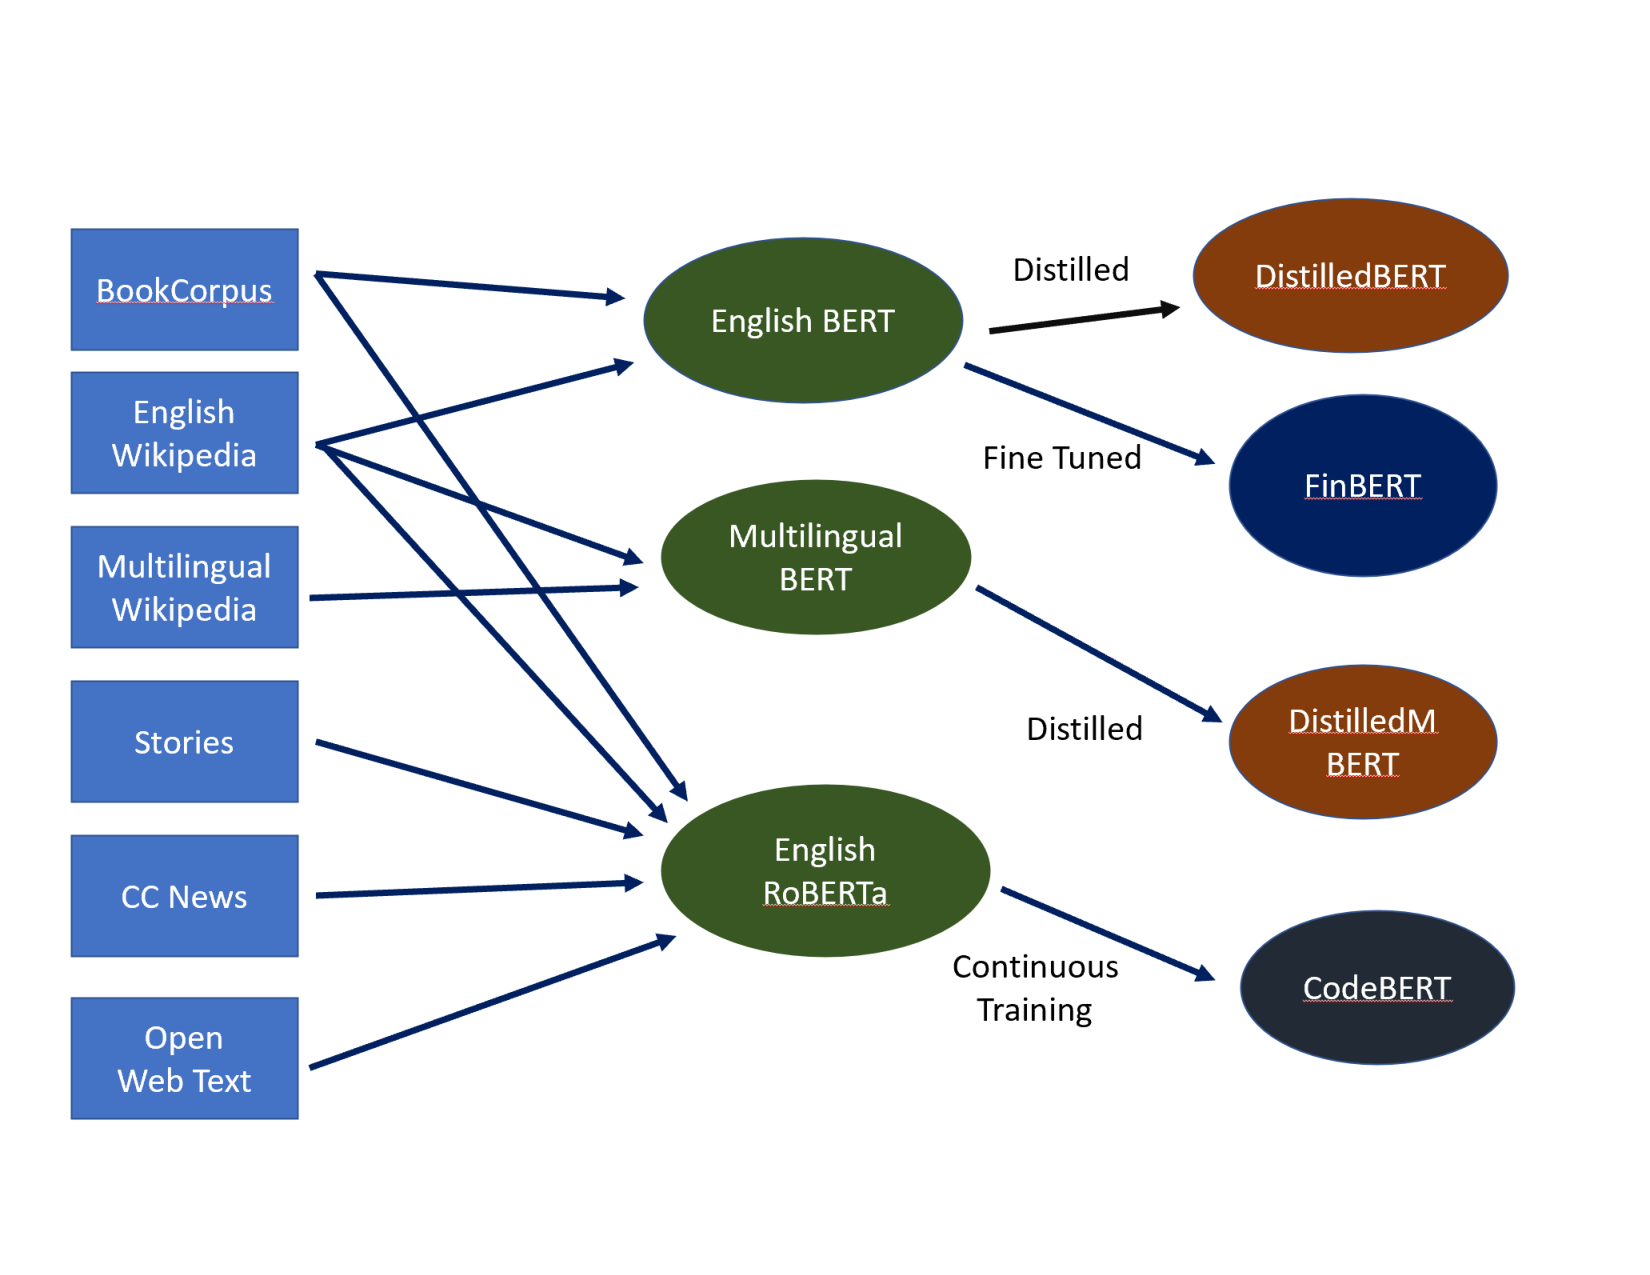
\includegraphics[width=8cm]{model-2.pdf}}
%%\caption{The 'Supply Chain' of data-sets and models}
%%  \label{fig:model-life-cycle}
%%\end{figure*}

\begin{figure}[]
\centering{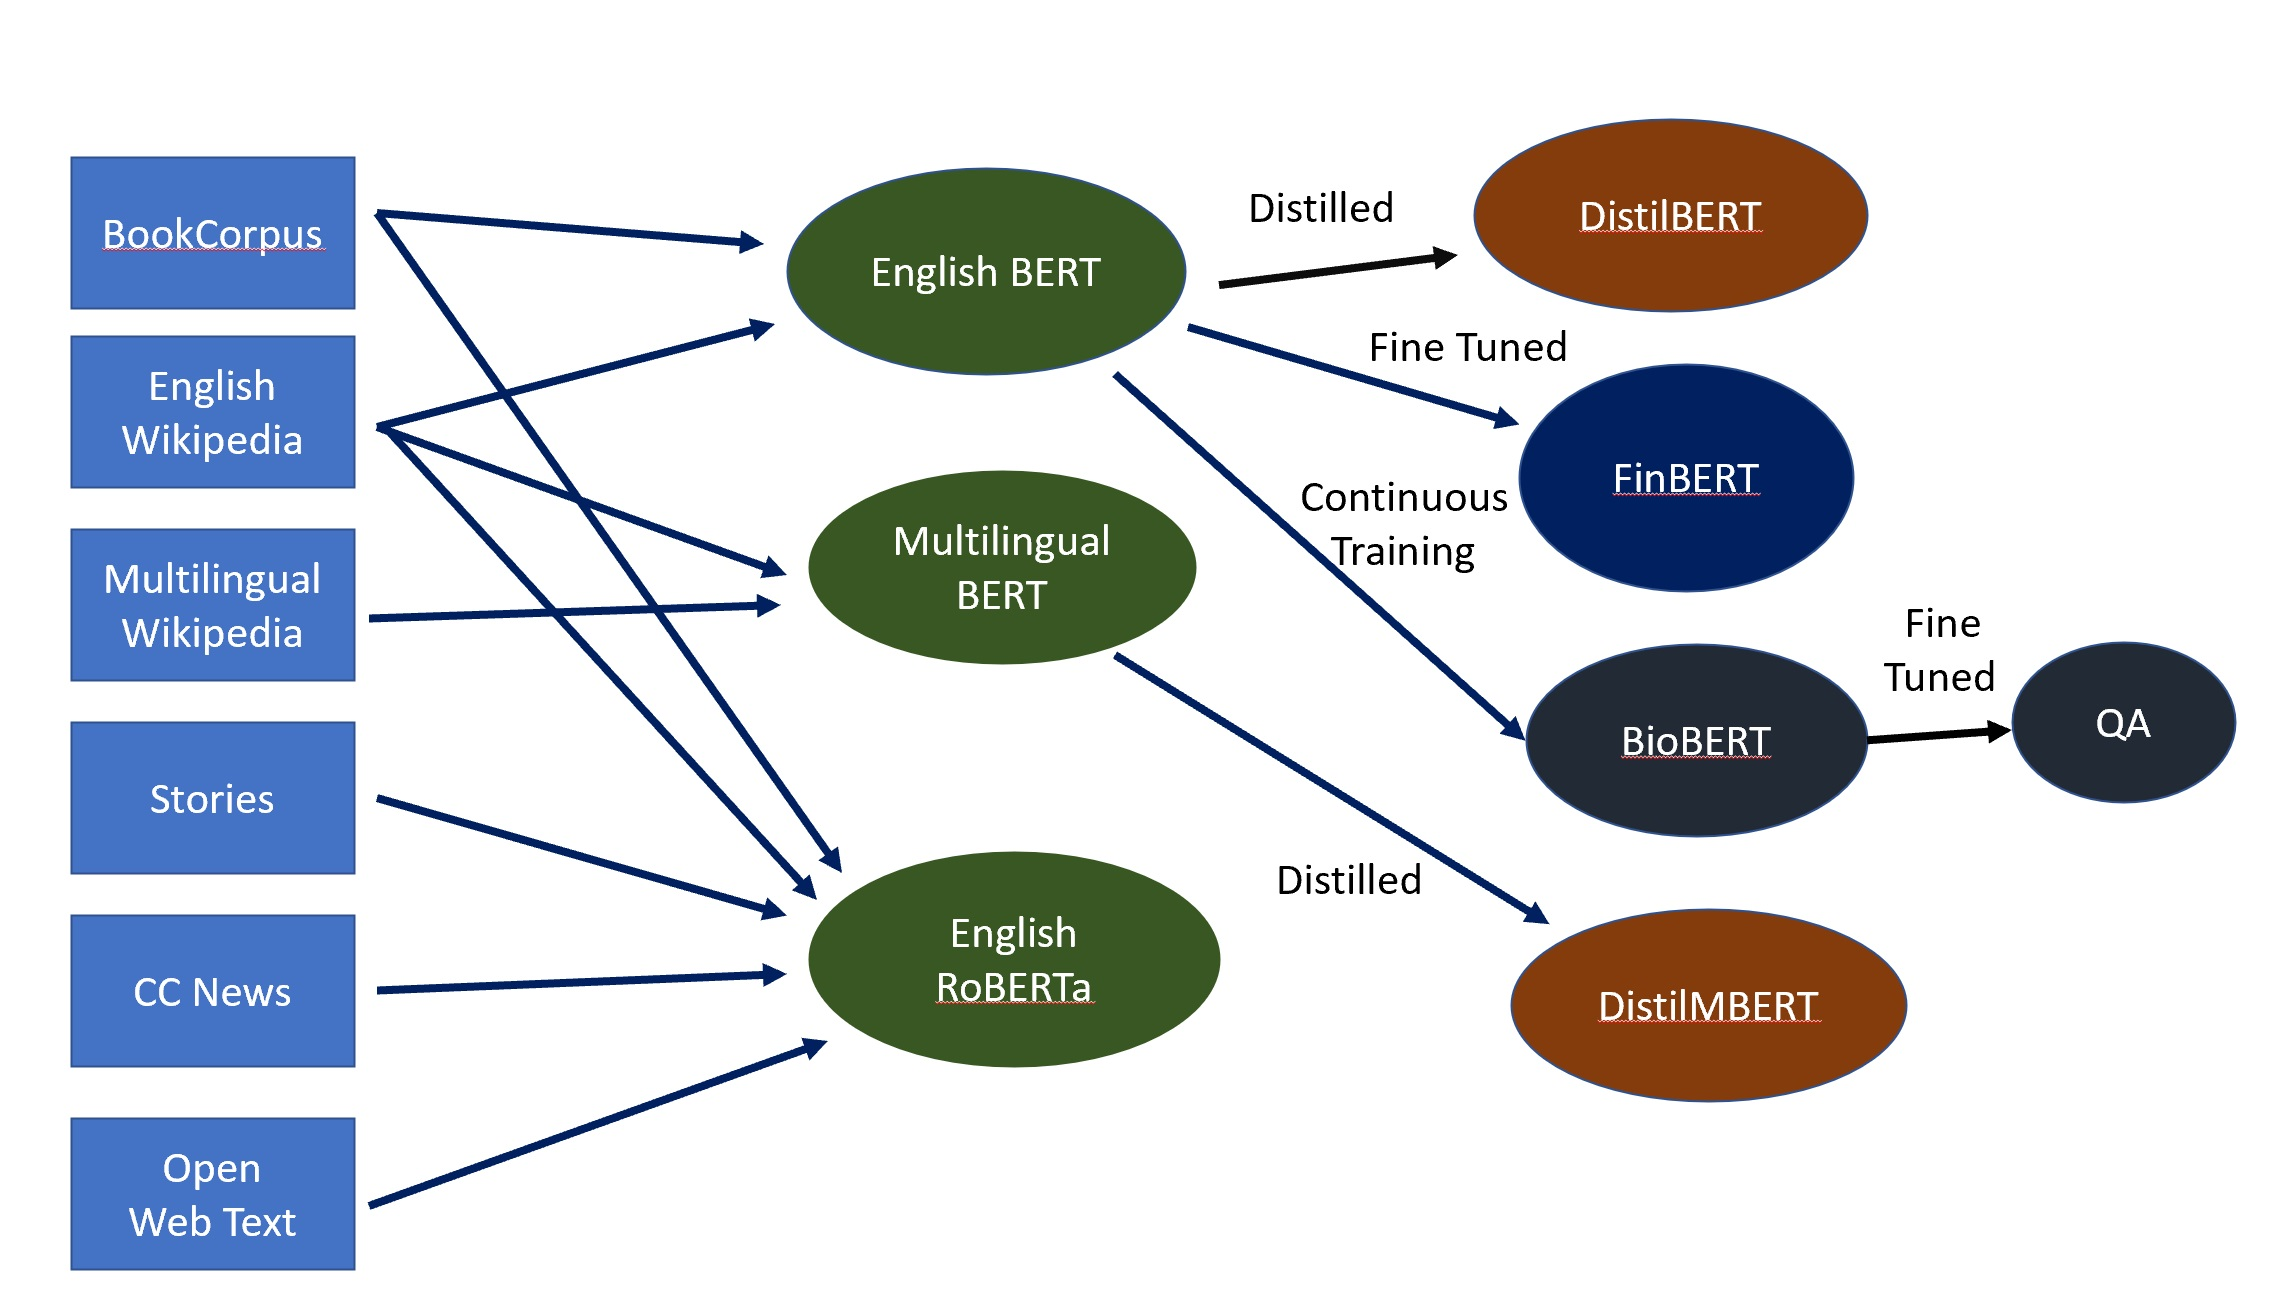
\includegraphics[width=8cm]{sustain1.jpg}}
\caption{The 'Supply Chain' of data-sets and models}
  \label{fig:model-life-cycle}
\end{figure}

A pre-processing pipeline, needed to curate data for training a model, could consist of the following steps: Data acquisition: via crawling (for NLP), or running simulations (materials or physics); De-duplicating:  to ensure there is one copy of a document from multiple sources; Selecting documents of certain languages of interest; Splitting the documents into sentences for training; Identifying Hate Abuse Profanity and PII information one may want to filter; Forming the data files for training based on a given format. For example, NLP datasets such as  Wikipedia,  Stories,  OpenWebText, BookCorpus, CC News are constructed via web crawling. 
Each of them could potentially be processed through all the above steps before it is ready for being used for training.  Fig. \ref{fig:model-preprocess} shows such a pipeline. 
 \begin{figure}[]
\centering{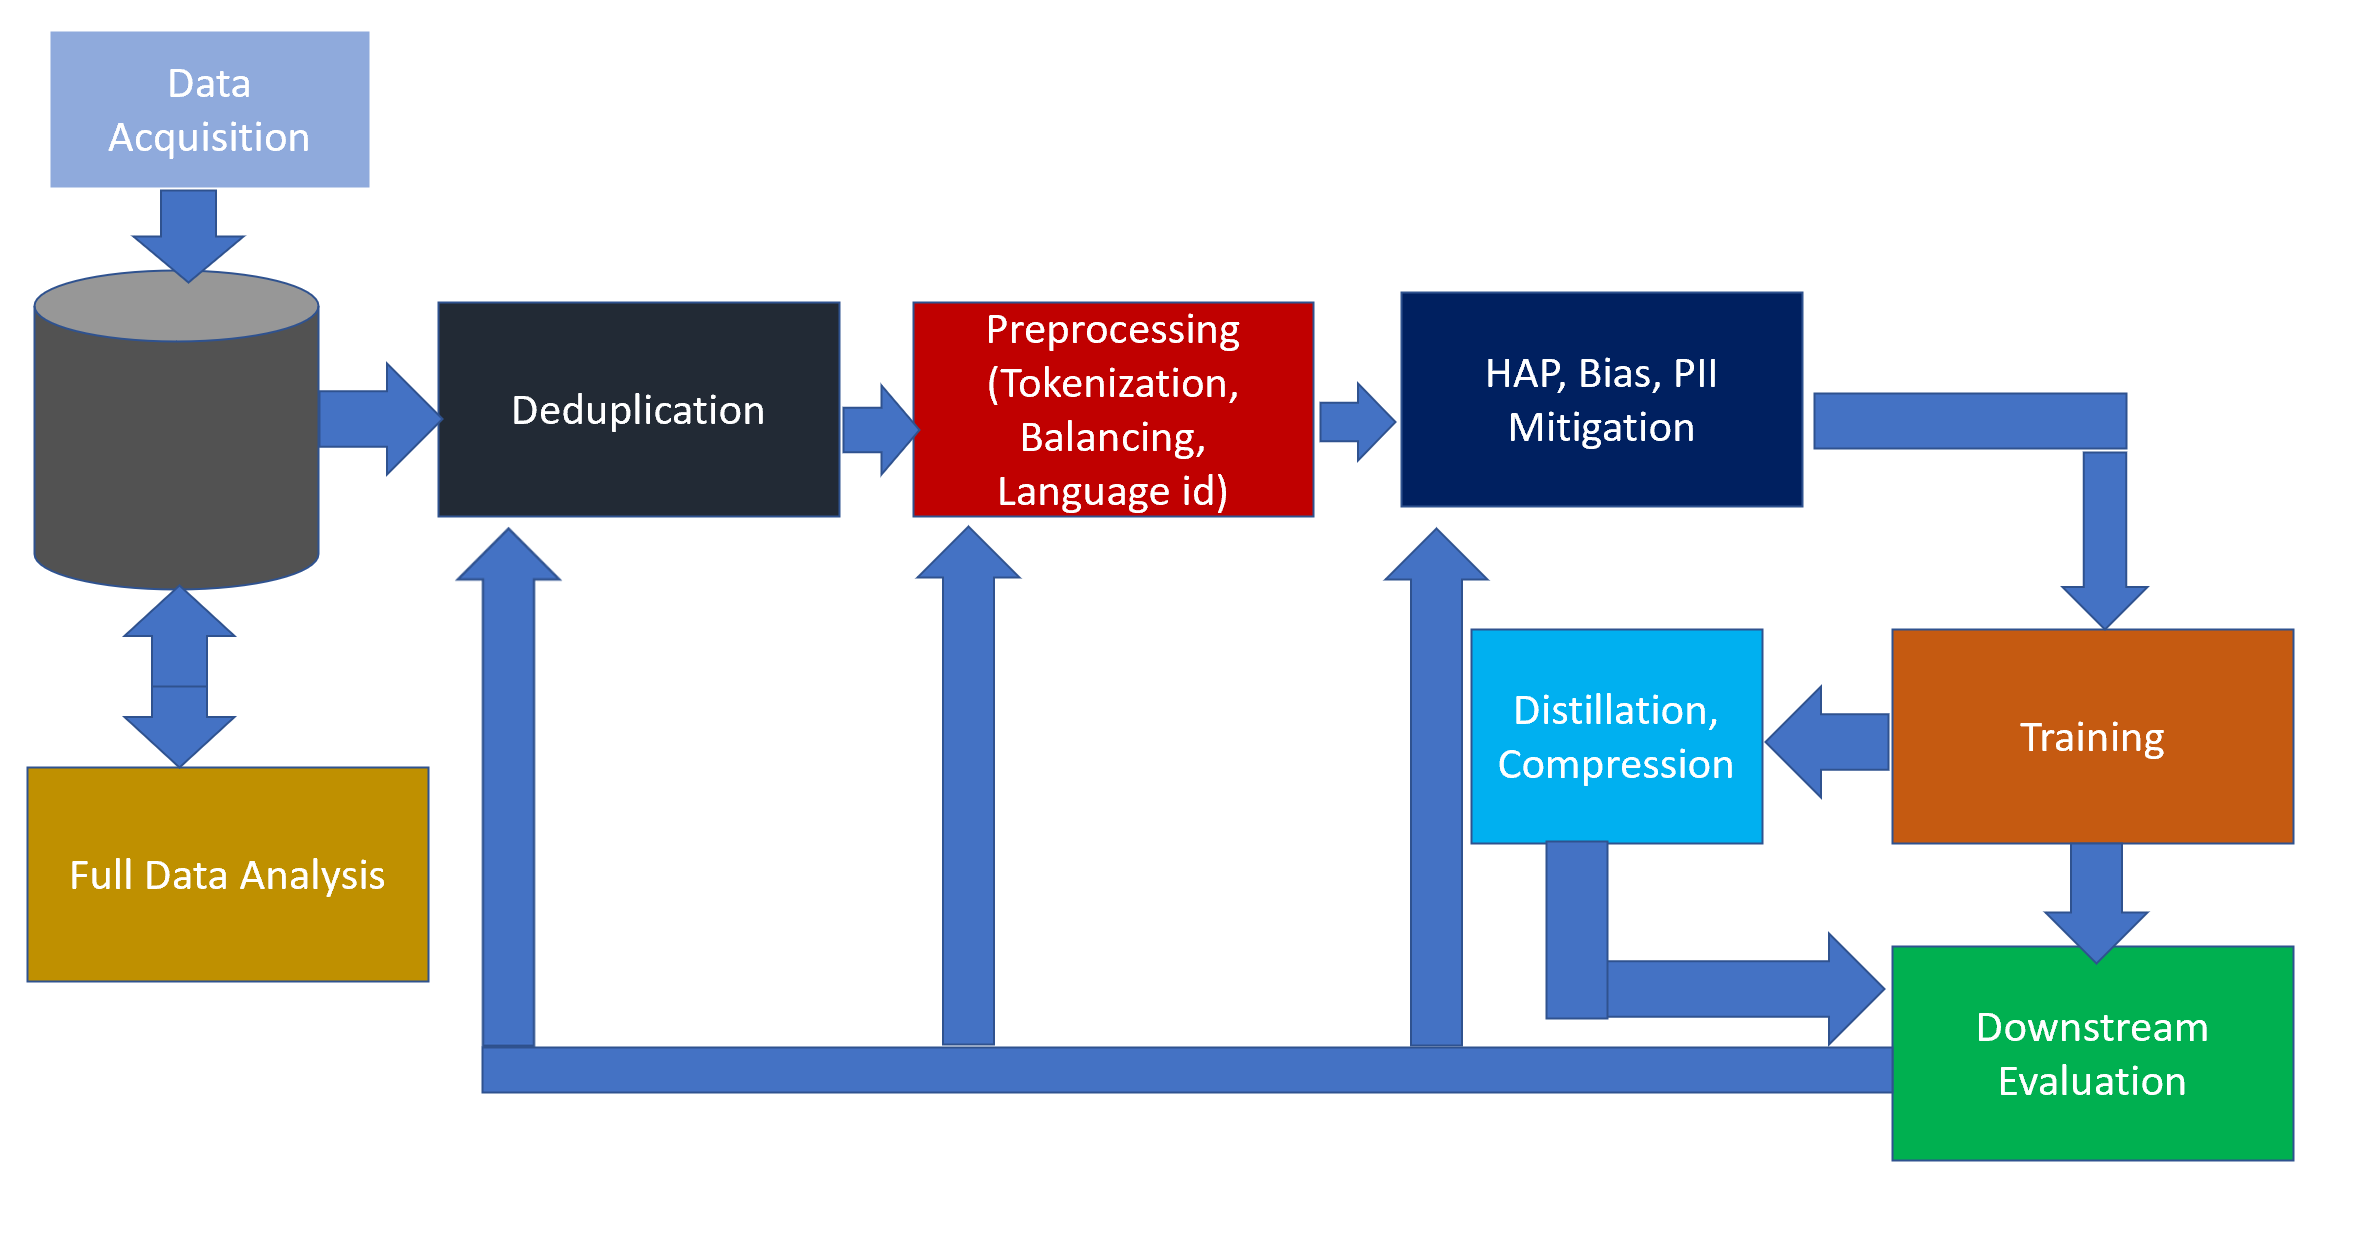
\includegraphics[width=8cm]{sustain3.png}}
\caption{A typical preprocessing pipeline}
  \label{fig:model-preprocess}
\end{figure}
The data-sets are used to train multiple models in various combinations. BERT, for example, was trained using English Wikipedia and BookCorpus. Whereas Multilingual BERT (mBERT) was trained on multilingual Wikipedia over 100+ languages \cite{DBLP:journals/corr/abs-1911-03310}.   RoBERTa on English data-sets spanning Wikipedia, Stories, OpenWebText, BoockCorpus as well as CC-News.  
%The effort needed to curate this datasets gets amortized over multiple models which benefit from it in various proportions - will get to this later
%
%In some instances a model needs to be oriented towards a certain domain by continuously training it further in unsupervised manner.  For example,  BioBERT \cite{DBLP:journals/corr/abs-1901-08746} was continuously trained on the biomedical domain on top of BERT. It was then finetuned for various tasks like Question Answering (QA).

After a model is trained, the model may be distilled to bring it to a form factor which fits certain latency or space budget. For example  DistilBERT \cite{DBLP:journals/corr/abs-1910-01108}and DistilMBERT are based on BERT and mBERT respectively.  
%They are of 6 layers instead of the 12 layers in BERT, and has $40\%$ less parameters then BERT base uncased; it runs $60\%$ faster while preserving $95\%$ pf the accuracy of BERT base on GLUE benchmark.
After the base model is deployed, if often needs to be continuously trained to maintain accuracy. A model trained before 2019 would not have known about COVID. The frequency of re-training varies. For example, 
~\cite{Wu2022} reported re-training in weekly, or daily
frequency for two different use cases. 
%Bhatta: I like to stress here post deployment continuous %training to keep a model such as recomendation or search %accurate. 
%FinBERT was created by fine-tuning a BERT model on finance data and CodeBERT was created by continuously training RoBERTa over github repositories. FinBERT delivers better result than the base BERT on financial analysis benchmarks like FiQA Sentiment Scoring and Financial Phrasebank. There is some additional effort needed for fine-tuning and continuous training to produce these models.
%The effort needed to create the BERT base is now not only utilized when BERT is used directly on any task but also when models spun off from it are also utilized.